\documentclass[varwidth,convert={density=500,size=1080x800,outext=.png}]{standalone}
\usepackage{mathtools}
\usepackage{graphicx}
\usepackage{bm}
\usepackage{color}
\usepackage[dvipsnames,table]{xcolor}
\usepackage{tikz}
\usepackage{stanli}
\usepackage{verbatim}
\usepackage{tikz}
\usetikzlibrary{shapes,calc,through,3d,patterns}
\usetikzlibrary{decorations.pathreplacing}
\usepackage{pgfplots}
\usepackage{siunitx} % For formatting numbers
\usepackage{hyperref}
\hypersetup{colorlinks=true,linkcolor=darkred}
\usepackage{multicol}
\usepackage[absolute,overlay,]{textpos}
\usepackage{pgfplots}
\pgfplotsset{width=10cm,compat=1.9}
\usepackage{subcaption}
\usepackage{multirow}
\usepackage{bbding}
\usepackage{arydshln}
\usepackage{mathtools}
\usepackage{tcolorbox}

\usepackage[dvipsnames]{xcolor}

\begin{document}
  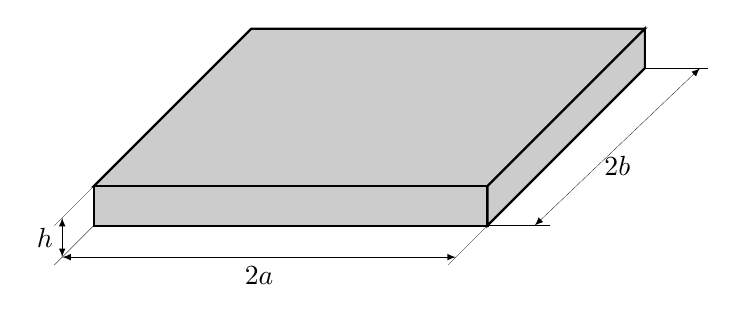
\begin{tikzpicture}
  \def\h{0.5}
    % lenght x
    \draw[ultra thin] (0,-\h) -- (-0.5,-0.5-\h);
    \draw[ultra thin] (5,-\h) -- (4.5,-0.5-\h);
    \draw[ultra thin,latex-latex] (-0.4,-0.4-\h) -- (4.6,-0.4-\h) node[midway, below]{$2a$};
    % lenght y
    \draw[ultra thin] (5,-\h) -- (5.8,-\h);
    \draw[ultra thin] (7,2-\h) -- (7.8,2-\h);
    \draw[ultra thin,latex-latex] (5.6,-\h) -- (7.7,2-\h) node[midway, below]{$2b$};
     % height
    \draw[ultra thin] (0,0) -- (-0.5,-0.5);
    \draw[ultra thin,latex-latex] (-0.4,-0.4-\h) -- (-0.4,-0.4) node[midway, left]{$h$};
    % Draw the rectangle (domain)
    \filldraw[fill=gray!40, draw=black,thick]  (0,0) -- (5,0) -- (7,2) -- (2,2) -- cycle;
    \filldraw[fill=gray!40, draw=black,thick]  (0,0) -- (5,0) -- (5,-\h) -- (0,-\h) -- cycle;
    \filldraw[fill=gray!40, draw=black,thick]  (5,0) -- (7,2) -- (7,2-\h) -- (5,-\h) --cycle;
  \end{tikzpicture}
  \end{document}